\documentclass{article}
\usepackage{fancyhdr,geometry,subfig,hyperref,graphicx,psfrag,amsfonts,wrapfig,mathtools}
\title{Mandatory exercise 2 \\ Signal and Image Processing 2012}
\author{Jens P. Raaby \\
\url{frn617@diku.dk}}

\begin{document}
\maketitle

\section*{Question 2.1 - Filtering Function}
I have implemented a simple Fourier-domain filtering package as a MATLAB function, applyFilter. This takes as parameters the image (in the form of a matrix), a filter (either spatial, in which case it will be Fourier transformed, or Fourier)  as well as a boolean option to visualise.

The steps taken by the applyFilter function are as follows:
The input image is converted to a matrix of double precision numbers. It's size is calculated and from that the padding size is also found (giving a padded size which is 4 times larger than the original). Then a padded version of the image is created (all outside areas are set to have a value of 0), and this is Fourier transformed.

Subsequently the filter is checked - if it is in the spatial domain the Fourier transform is calculated and shifted such that the filter is symmetric and padded to the same size as the padded image. 

Filtering is performed by multiplying each pixel with the corresponding filter value, both of which are in the Fourier domain. To retrieve the filtered image, the result of the previous multiplication is inverse-Fourier transformed and the imaginary part is discarded. The padding is removed to yield an image with the same dimensions as the original.

If the `visualise' parameter was set when calling the function, a table of images is presented to the user with the image, filter and resulting image shown in both the frequency and spatial domains.

For generating the averaging filter (in the spatial domain), a simple 5 x 5 matrix of ones is first created. The values are then scaled by $\frac 1 {25}$. The ideal low pass filter is created directly in the Fourier domain form. It creates a circle of radius $D_0$ (the cutoff frequency).

\subsection*{Results}
The original and filtered versions of `testimg.tif' are shown in figure \ref{fig:q21}. The 5 x 5 averaging filter creates a slightly blurred version of the image (figure \ref{fig:1b}), and the zero-padding has created a black edge on the top and left sides.
Applying the ideal low pass filter (with a cutoff frequency of 50) also gives a slightly blurred image (figure \ref{fig:1c}) but it also has `halo' artefacts near edges. It has added some frequency noise in this instance, if one inspects the areas which were originally plain grey.
\begin{figure}[h]
\centering
	\subfloat[Original Image]{\label{fig:1a}
\includegraphics[width=0.3\textwidth]{q1-originaltest.png}}\qquad
	\subfloat[5 x 5 Averaging filter]{\label{fig:1b}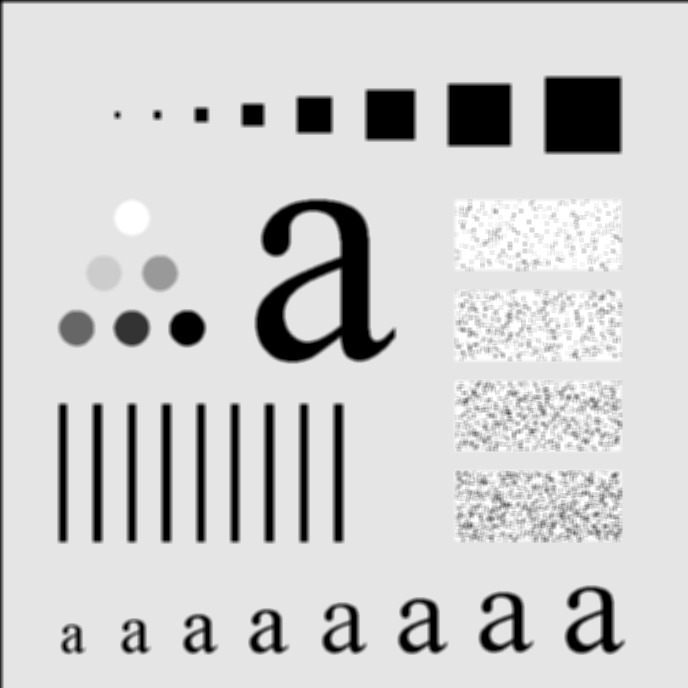
\includegraphics[width=0.3\textwidth]{q1-averagedtest.png}}\qquad
	\subfloat[Ideal low pass filter ($D_0=50$)]{\label{fig:1c}
\includegraphics[width=0.3\textwidth]{q1-lptest.png}}
	\caption{Filtering the test image for question 2.1}
	\label{fig:q21}
\end{figure}


\section*{Question 2.2 - Gaussian filters}
For this question I implemented a function `gaussianLowPass' which creates a Gaussian Low Pass filter with the given size P x Q and cutoff frequency $D_0$. I used the definition given in Gonzalez and Woods section 4.8.3. This filter can be also be used to create High Pass filters by subtracting the matrix from 1, and thus also for the High-frequency-emphasis filter.

\subsection*{Low Pass}
Varying the cutoff frequency ($D_0$) with the Gaussian low pass yields the results shown in figure \ref{fig:q221} on the image `barbara.tif'.
\begin{figure}[h]
\centering
	\subfloat[$D_0=50$]{\label{fig:221a}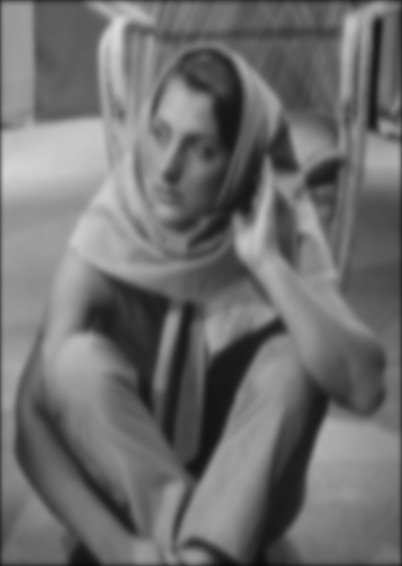
\includegraphics[width=0.2\textwidth]{q2-lowpass-50.png}}\qquad
	\subfloat[$D_0=100$]{\label{fig:221b}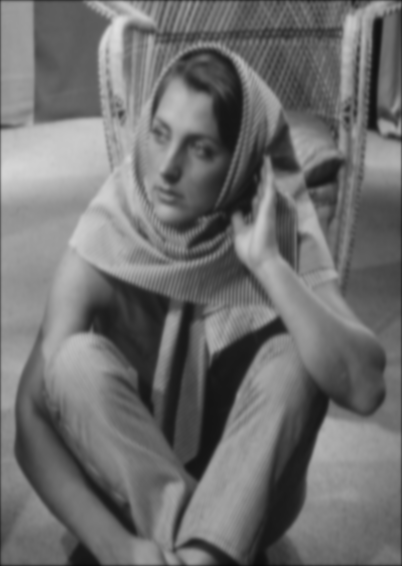
\includegraphics[width=0.2\textwidth]{q2-lowpass-100.png}}\qquad
	\subfloat[$D_0=150$]{\label{fig:221c}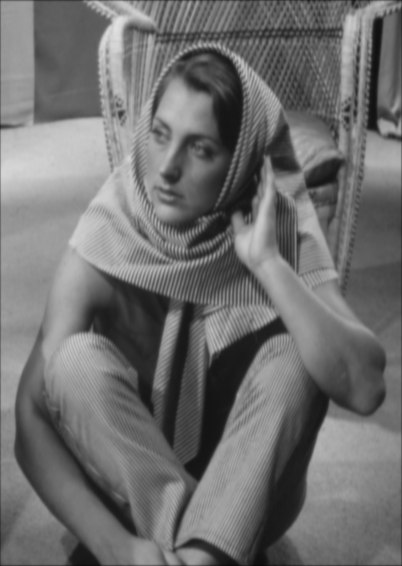
\includegraphics[width=0.2\textwidth]{q2-lowpass-150.png}}\qquad
	\subfloat[$D_0=200$]{\label{fig:221d}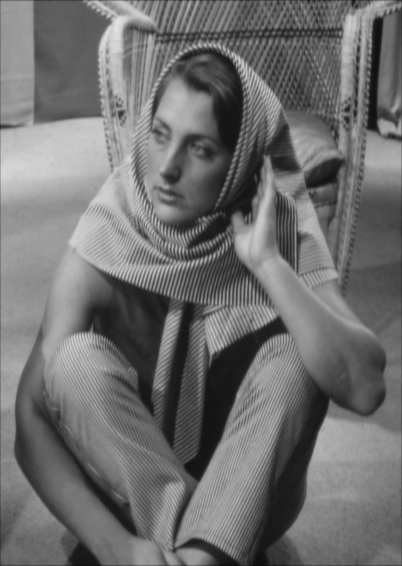
\includegraphics[width=0.2\textwidth]{q2-lowpass-200.png}}\qquad
	\caption{Gaussian Low Pass with varying $D_0$}
	\label{fig:q221}
\end{figure}
Clearly, the apparent sharpness of the filtered image increases as the cutoff frequency increases. The low pass filter essentially removes frequencies above the cutoff value. Therefore if it is set low, nearly all higher frequency details will be ``cut off''. As the cutoff reaches the maximum, more and more details are included in the filtered image.
In figure \ref{fig:221a} the image appears soft, but Barbara is still recognisable. If an object-detection algorithm ran on this image it would not be too impaired by high frequency patterns (for example on the trousers.) The final image in the series includes nearly all the patterns on the trousers and scarf, and this could cause problems for some algorithms.

\subsection*{High Pass}
\begin{figure}[h]
\centering
	\subfloat[$D_0=50$]{\label{fig:222a}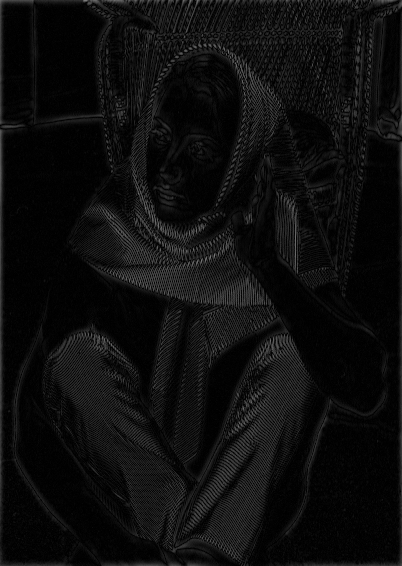
\includegraphics[width=0.2\textwidth]{q2-highpass-50.png}}\qquad
	\subfloat[$D_0=100$]{\label{fig:222b}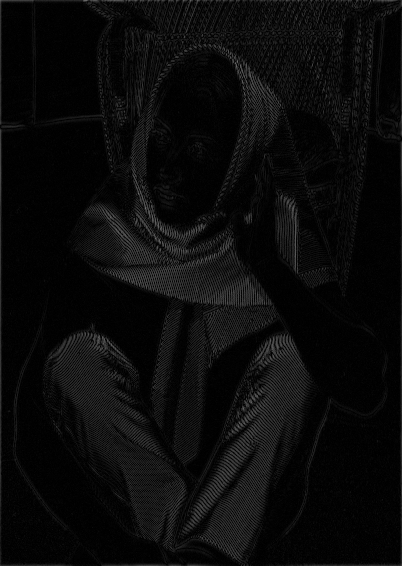
\includegraphics[width=0.2\textwidth]{q2-highpass-100.png}}\qquad
	\subfloat[$D_0=150$]{\label{fig:222c}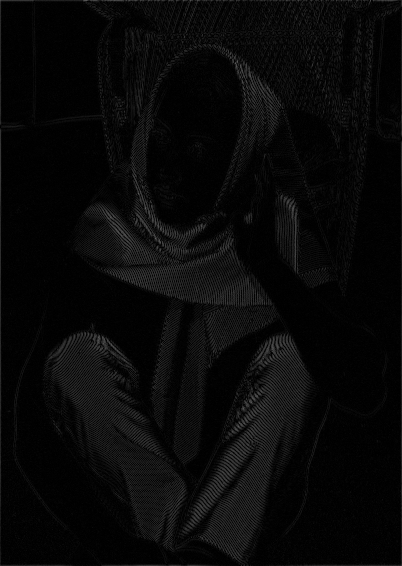
\includegraphics[width=0.2\textwidth]{q2-highpass-150.png}}\qquad
	\subfloat[$D_0=200$]{\label{fig:222d}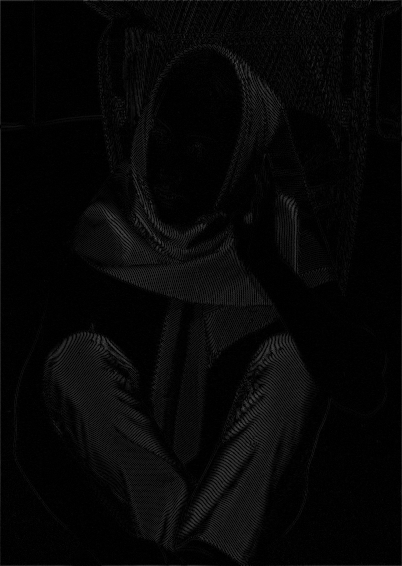
\includegraphics[width=0.2\textwidth]{q2-highpass-200.png}}\qquad
	\caption{Gaussian High Pass with varying $D_0$}
	\label{fig:q222}
\end{figure}

Rather than filtering out high frequencies like the Low Pass filter, the Gaussian High Pass filter removes low frequency detail. The larger the value of the cutoff $D_0$, the more low frequency details are removed. Looking closely at figure \ref{fig:q222}, it can be seen that fewer details are included as $D_0$ increases. The facial details are already removed at $D_0 = 100$ and it is mainly fabric detail which remains in the final image.

\subsection*{High-frequency emphasis}
The high-frequency-emphasis (HFE) filter is a function of the Gaussian High Pass filter: $1 + k * H_{hp} (u,v)$ (section 4.9.5 in Gonzalez and Woods).
The parameter k determines whether the filter acts as an `unsharp mask' or a `high boost' filter.

The name of the filter suggests that this filter will enhance the presence of fine details in an image. Therefore, in theory, if an image has had the high frequency detail removed (for example by a Low Pass filter) then the HFE filter will emphasise the remaining fine details. It cannot `bring back' fine details that have been cut off, but can exaggerate those which remain.

The result of applying the HFE filter ($k=1$) to the image of Barbara in figure \ref{fig:221b}  ($D_0 = 100$) is shown in figure \ref{fig:223b}. The result is a slight sharpening, but the image is not restored to the same level as the original, shown in figure \ref{fig:223c}. In particular, the trousers are lacking texture. On the other hand, some of the background detail has been restored by the filtering, and Barbara's face is noticeably sharper. Increasing the value of $k$ (creating the High Boost filter) does appear to recover more sharpness, as shown in figure \ref{fig:223d}. There are more artefacts and a slight jaggedness, but the image looks better next to the original when this document is downscaled (there appears to be a Moir� pattern on my computer). The facial details actually appear sharper in \ref{fig:223d} than in the original, whereas the higher frequency details which were removed by the low pass (for example the trouser pattern) are pleasingly smoothed.
\begin{figure}[h]
\centering
	\subfloat[Low pass $D_0 = 100$]{\label{fig:223a}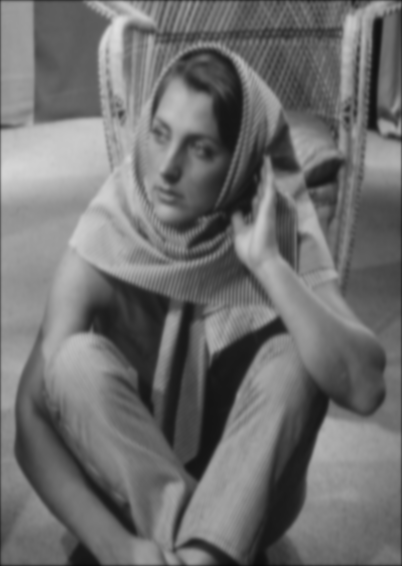
\includegraphics[width=0.2\textwidth]{q2-lowpass-100.png}}\qquad
	\subfloat[`Unsharp mask' HFE applied to the low pass image ($k=1$, $D_0 = 100$)]{\label{fig:223b}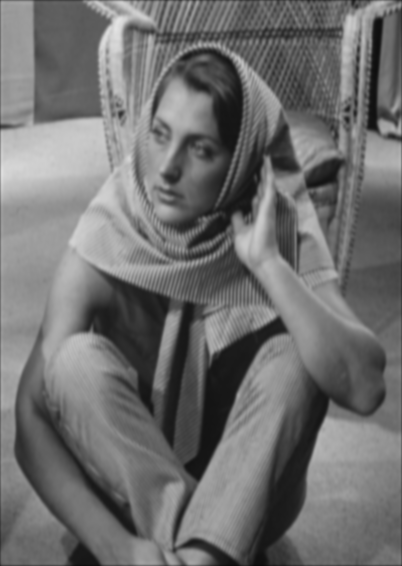
\includegraphics[width=0.2\textwidth]{q2-hfe-100.png}}\qquad
	\subfloat[`High boost' HFE ($k=3$, $D_0 = 100$) ]{\label{fig:223d}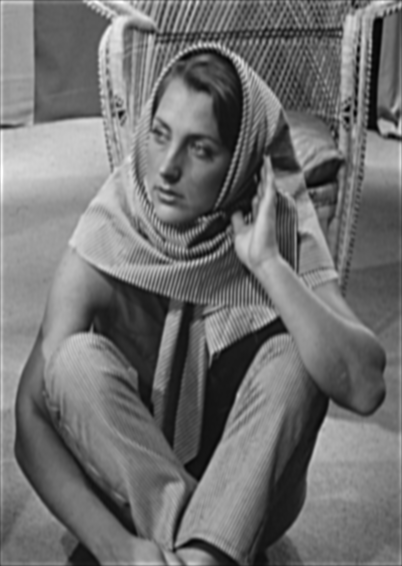
\includegraphics[width=0.2\textwidth]{q2-hfe-k3-100.png}}\qquad
	\subfloat[Original image]{\label{fig:223c}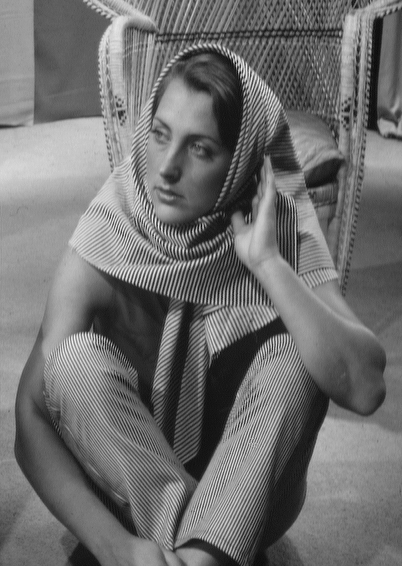
\includegraphics[width=0.2\textwidth]{q2-barbara.png}}
	\caption{Gaussian High Frequency Emphasis applied to a Low Pass filtered image}
	\label{fig:q223}
\end{figure}


\section*{Question 2.3 - Image resampling}
\subsection*{Downsampling}
Taking the naive approach of discarding rows and columns between every 4th row and column, the result shown in figure \ref{fig:231a} was obtained. Note the aliasing patterns which were not present in the original. I next removed the high frequency detail using a Gaussian low pass filter before applying the same reduction. The result is shown in figure \ref{fig:231b} and the similar result after using the 5 x 5 averaging filter is in figure \ref{fig:231c}. These two reductions are noticeably blurry compared to the naive reduction. I then tried applying an unsharp mask to the Gaussian low pass filtered reduction, resulting in figure \ref{fig:231d}. This version has recovered the appearance of sharpness which the former conversions lost. I experimented with values for $D_0$ and fount that above a certain value (~75) no further sharpness could be achieved, but below ~40 the smoother areas of the image gain in contrast and don't resemble the original resolution image.

\begin{figure}[h]
\centering
	\subfloat[Simple reduction]{\label{fig:231a}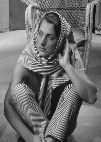
\includegraphics[width=0.2\textwidth]{q3-shrunk-aliased.png}}\qquad
	\subfloat[Gaussian Low Pass before reduction  ($D_0 = 100$)]{\label{fig:231b}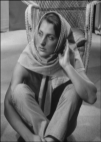
\includegraphics[width=0.2\textwidth]{q3-shrunk-anti-aliased-1.png}}\qquad
	\subfloat[5x5 averaging applied before reduction]{\label{fig:231c}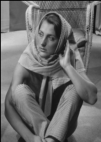
\includegraphics[width=0.2\textwidth]{q3-shrunk-anti-aliased-2.png}}\qquad
	\subfloat[Gaussian LP before downsampling, HFE with $D_0 = 50, k =1$ after]{\label{fig:231d}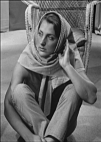
\includegraphics[width=0.2\textwidth]{q3-shrunk-anti-aliased-3.png}}
	\caption{Gaussian High Frequency Emphasis applied to a Low Pass filtered image}
	\label{fig:q223}
\end{figure}
\subsection*{Upsampling}

\section*{Question 2.4}
\subsection*{Interference patterns}
\subsection*{}
\end{document}